\section{Exercise 2: Recognize Design Patterns}

First of all, please find below a simplified class diagram to visualize
more easily how the different classes interact.\\

\begin{figure}[h!]
    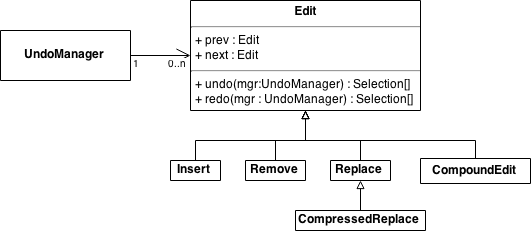
\includegraphics[width=0.8\textwidth]{images/ex2.png}
    \centering
    \caption{Exercise 2 Class Diagram}
\end{figure}

The inner classes \emph{Edit}, \emph{Insert}, \emph{Remove}, \emph{Replace},
\emph{CompressedReplace}, \emph{CompoundEdit} are part of an implementation of
the Command design pattern which is a behavioral pattern. \emph{Edit} is an
abstract class that all commands inherits. Each command must implement an
\emph{undo()} and a \emph{redo()} action. By using this pattern, each operation
applied to a buffer (e.g. inserting text, removing text) is instantiated
as a class implementing the \emph{Edit} interface so that they can be
easily saved in queues in order to \emph{undo()} or \emph{redo()} them.
Without this pattern, undo and redo could be implemented by saving the
content of the buffer after each operation, but that would be more
expensive memory-wise.\\

The \emph{Edit} abstract class and its children are part of a composite
design pattern, which is a structural pattern. In this implementation,
there are no leafs, only composite elments (\emph{Edit} and its
children). This pattern is used here in order to retrieve the previous
and next \emph{Edit}, which is useful for implementing the redo and undo
queues.
\newpage
